%%%%%%%%

\chapter{Presentation of \tafkit}
\label{chp:shr-prs-tfk}


\tafkit stands for \emph{Typed Automata Function Kit};
it is a \emph{command-line interface} to \vcsn.
As stated in the introduction, the \vcsn platform is dedicated to the 
computation of, and with, finite automata, where `finite automata' means 
\emph{weighted automata} over \apriori \emph{arbitrary monoids}.

In the static generic programming paradigm used in the \vcsn library, the
\emph{types} of the automata that are treated have to be known at 
compile time. 
\tafkit, which is a set of programs
that should be called from the \code{shell} and that can be used to chain
operations on automata, has therefore been compiled for several 
predefined types of automata.
It thus allows to use \emph{already programmed} functions on automata of 
\emph{predefined types}.
\tafkit gives a \emph{restricted access} to \vcsn functionalities, 
but it is a \emph{direct access}, without any need of programming 
skill.
A basic familiarity with Unix command syntax only is sufficient to make 
use of \tafkit.

In this chapter, we first give a series of examples of commands in 
the case of `classical automata'.
We then present the overall organisation of \tafkit, with the list of 
possible instances and options.
The following section describes the syntax of options that help 
define the behaviour of the commands whereas the fourth section 
describes the syntax of rational (\ie regular) expressions within 
\vcsn.
The final section lists the input--output commands of \tafkit;
all other commands are presented in the next chapter.


\section{First contact}
\label{sec:fir-con}

Let us first suppose that \vcsn is fully installed (as explained in 
\secti{bui-ld}).\footnote{%
    If \vcsn is only compiled without being installed, 
    one should first go to the 
    \file{vaucanson-\VcsnVersion/taf-kit/tests/} directory by a 
    \command{cd} command, 
    and type
    \samp{./vcsn-char-b} instead of \samp{vcsn-char-b} for each of the
    following commands.}
Any of the following commands could be typed and their results observed.
 
We describe now (some of) the functions of the instance of \tafkit 
which deals with `classical automata', \ie \emph{Boolean automata} 
over a free monoid whose generators are \emph{characters}.
These functions are called by the \command{vcsn-char-b} command.

To begin with, we have to deal with an automaton of the correct type.
There are several means to build or define such an automaton, but the 
most direct way is to use one of those whose definition comes with 
\tafkit.
We choose the automaton $\Ac_1$ shown at \figur{a1} 
and whose description is contained in the \xml 
file \file{a1.xml}. 



\begin{figure}[ht] 
    \centering
% \begin{center}
\VCDraw{%
\begin{VCPicture}{(-1.4,-1.4cm)(7.4,1.4cm)}
% etats[p][r][q]
\State{(0,0)}{A}\State{(3,0)}{B}\State{(6,0)}{C}
%
\Initial{A}\Final{C}
% transitions 
\EdgeL{A}{B}{a}\EdgeL{B}{C}{b}
%
\LoopN{A}{a}\LoopS[.22]{A}{b}
\LoopN{C}{a}\LoopS[.22]{C}{b}
%
\end{VCPicture}}
% \end{center}
    \caption{The Boolean automaton $\Ac_1$ over 
    $\{a,b\}^{*}$. }
\label{fig:a1}
\end{figure}
%  recognizes any word that contains $ab$
 
The first command \command{data} will just make sure that \tafkit knows about
this automaton.  It will display the number of states, transitions,
initial states, and final states of $\Ac_1$.

\begin{shell}
$ \kbd{vcsn-char-b data a1.xml}
States: 3
Transitions: 6
Initial states: 1
Final states: 1
\end{shell}%$

This automaton \file{a1.xml} can also be displayed with the command 
\command{display}:\footnote{%
   If the \code{GraphViz} package is installed (see \secti{pre-req}).}

\begin{shell}
$ \kbd{vcsn-char-b display a1.xml}
\end{shell}%$

The displayed automaton won't have a layout as pretty as in
\figur{a1}, but it represents the same automaton nonetheless.

\begin{figure}[ht]
    \centering
\includegraphics[scale=0.5]{figures/imm1.ps}
\caption{Result of the command \code{vcsn-char-b display a1.xml}}
\label{fig:a1}%
\end{figure}

The command \FctInd{aut-to-exp} outputs a rational expression which 
denotes the language accepted by $\Ac_1$.
The command \FctInd{eval} tells whether a word belongs to that 
language (answer with \code{1} = yes, or \code{0} = no).
This is not to be confused with a function with a Boolean answer... 
\cf \sbsct{boo-res-for}.

\begin{shell}
$ \kbd{vcsn-char-b aut-to-exp a1.xml}
(a+b)*.a.b.(a+b)*
$ \kbd{vcsn-char-b eval a1.xml 'babab'}
1
\end{shell}%$

The automaton $\Ac_1$ is not deterministic and the 
\command{determinize} command will compute its determinisation. 
As most \tafkit commands, \command{determinize} produces its output 
(an \xml file representing the automaton) on the standard output, an 
event which would hardly be of interest.
The normal usage is to divert the output by means of a \code{shell} 
redirection to a file for subsequent computation with other commands.

\begin{shell}
$ \kbd{vcsn-char-b determinize a1.xml > a1det.xml}
$ \kbd{vcsn-char-b data a1det.xml}
States: 4
Transitions: 8
Initial states: 1
Final states: 2
$ \kbd{vcsn-char-b display a1det.xml}
\end{shell}%$

\begin{figure}[ht]
    \centering
\includegraphics[scale=0.4]{figures/a1det.ps}
\caption{The determinisation of \code{a1.xml}}
\label{fig:a1-det}%
\end{figure}

The file \file{a1det.xml} has been created into
the current directory while \file{a1.xml} is a file that is predefined
in \vcsn's predefined automata repository.  
We can call the command
\command{data} on either files using the same syntax because \tafkit
will look for automata in both places.  

% The command \samp{vcsn-char-b  list-automata} will list all 
% predefined automata for this instance 
% of \tafkit.  See also \chptr{aut-rep-fac} for a presentation
% of these files.

In the pure Unix tradition, we can of course chain commands with
pipes.  
\index{pipe!shell --}%
For instance, the above two commands could be rewritten as:

\begin{shell}
$ \kbd{vcsn-char-b determinize a1.xml | vcsn-char-b data -}
States: 4
Transitions: 8
Initial states: 1
Final states: 2
\end{shell}%$
\noindent
where \samp{-} stands for `\emph{read from standard input}'.


\tafkit actually supports a more efficient way of chaining commands:
the \emph{internal pipe}.  
\index{pipe!internal --}%
\index{internal|see{pipe}}%
It is called \emph{internal} because
the pipe logic is taken care of by \tafkit itself, 
% but actually it is
and
not using a Unix pipe at all: the commands are simply serialized in
the same process, using the automata object created by the previous
one.  
It is more efficient because the automaton does not have to be
converted into an \xml file for output, and then parsed back as input of the
next command in the chain.  
Here is how the above command would look
using an \emph{internal pipe}; notice how the \samp{|} symbol is
protected from its evaluation by the shell.

\begin{shell}
$ \kbd{vcsn-char-b determinize a1.xml \bslash| data -}
States: 4
Transitions: 8
Initial states: 1
Final states: 2
\end{shell}%$

\noindent In the above command, \samp{-} does not designate the
standard input, it denotes \emph{the result of the previous command}.

\section{\tafkit organisation}
\label{sec:taf-org}%

\tafkit is indeed \emph{one program}, and this same program is
\emph{compiled} for different types of automata.  
The result of each compilation yields a command (with a distinct 
name) which can be called from the shell.
As we have seen in the preceding examples, every such command 
essentially takes two arguments: the first one determines a function and 
the second one an automaton which is the operand for the function.


\subsection{Automata types}
\label{ssc:aut-typ}%

A (finite) automaton is a (finite) directed  graph, labelled by 
\emph{polynomials} in~$\KPM$, that is, by (finite) \emph{linear 
combinations} of elements of a \emph{monoid}~$M$  
with coefficients in a \emph{semiring}~$\K$.
The \emph{type of an automaton} is thus entirely determined (in 
\vcsnv)\footnote{%
   We add this precision as in the next version \vcsn~2, the `kind' 
   of labels will also be a criterion in the definition of the 
   (programming) type of an automaton.} 
by the specification of~$\K$  and of the type of~$M$.
%

\subsubsection{Semirings}

The semirings that are instanciated in \tafkitv are 
shown in \tabla{srg-ins}. 
All these semirings are `numerical' in the sense their elements are 
implemented as numbers, but for the rationals: \code{float} for~$\R$,  \code{bool} 
for~$\B$,  \code{int} for the others.
The rationals are pairs of integers and implemented as pairs of an \code{int}
and an \code{unsigned}.
They all are \emph{commutative} semirings.

\begin{table}[ht]
\begin{center}
\begin{tabular}{llc}
\hline
\multicolumn{1}{c}{semiring} & mathematical symbol & suffix in \tafkit \\
\hline
Boolean semiring & $\msp\B = \StruSA{\B,\lor,\land}\msp$ & 
\samp{-b} \\
ring of integers & $\msp\Z = \StruSA{\Z,+,\times}\msp$ &
\samp{-z} \\
field of reals &$\msp\R = \StruSA{\R,+,\times}\msp$&
\samp{-r} \\
field of rationals &$\msp\Q = \StruSA{\Q,+,\times}\msp$&
\samp{-q} \\
two element field & $\msp\F_{2} = \StruSA{\{0,1\},+,\times}\msp$
	 (with $\msp 1+1 = 0\msp$)&
\samp{-f2} \\
min-tropical semiring & $\msp\Zmin = \StruSA{\Z,\min,+}\msp$&
\samp{-zmin} \\
max-tropical semiring  &$\msp\Zmax = \StruSA{\Z,\max,+}\msp$&
\samp{-zmax} \\
\hline
\end{tabular}
\end{center}
\caption{The semirings implemented in \vcsn \tafkitv}
\label{tab:srg-ins}
\end{table}



\subsubsection{Monoids}

The monoids instanciated in \tafkitv are 
the \emph{free monoids} and the \emph{direct products of (two) free monoids}. 
A free monoid is completely determined by the set of generators, called 
\emph{alphabet}.
At compile time however, it is not necessary to know the alphabet 
itself: the \emph{type} of its elements, the \emph{letters}, will 
suffice.
Thus, for \tafkit, the type of letters of one alphabet for a free monoid, 
of two alphabets for a 
direct product of two free monoids has to be defined.
In \tafkitv, the following types of letters are 
considered:
\begin{enumerate}
    \item  the \emph{simple} letters, which may be \emph{characters}: 
    \code{char}, or \emph{integers}: \code{int};

    \item  \emph{pairs} of simple letters.
\end{enumerate}
The combinations that are instanciated in \tafkitv is shown  in 
\tabla{mon-ins}.



\begin{table}[ht]
\begin{center}
\begin{tabular}{l>{\ttfamily\e}l>{\ttfamily\e}l}
\hline
\multicolumn{1}{c}{letter types} & 
\multicolumn{1}{c}{free monoids} & 
\multicolumn{1}{c}{free monoid products} \\
\hline
characters & char & char-fmp \\
integers & int & int-fmp \\
pair of characters & char-char\ee & \\
pair of integers & int-int & \\
pair of character and integer & char-int & \\
\hline
\end{tabular}
\end{center}
\caption{The monoids implemented in \vcsn \tafkitv}
\label{tab:mon-ins}
\end{table}

\subsection{\tafkit instances}
\label{ssc:taf-ins}%

As the consequence of the preceding subsection, the type of an 
automaton is determined by the following three data:
\begin{enumerate}
    \item  the type of the weight semiring;

    \item  the fact that the monoid is either a free monoid or a 
	product of two free monoids.
    
    \item the type of the letters that generate the free monoid(s).
\end{enumerate}

Not all possible combinations derived from the types of semiring and 
free monoid listed  above are instanciated (it would amount to over 70
possibilities --- even if one restricts oneself to the same type for 
the input and output monoids in transducers).
In \vcsnv, `only' 18 combinations are instanciated;
\tabla{tfk-ins} 
shows these instances, their names (that is, how they should 
be called from the \code{shell}), and the type of automata they allow 
to work with.

\begin{table}[ht]
\begin{center}
\begin{tabular}{lcl>\e l}
\hline
\multicolumn{1}{c}{program name} & 
\multicolumn{1}{c}{automaton type} & 
\multicolumn{1}{c}{alphabet type} & 
\multicolumn{1}{c}{weight semiring} \\
\hline
\command{vcsn-char-b} & automata &
  characters & $\langle\B,\lor,\land\rangle$ \\
\command{vcsn-int-b} & automata &
  integers & $\langle\B,\lor,\land\rangle$ \\
\command{vcsn-char-char-b} & automata &
  pairs of characters & $\langle\B,\lor,\land\rangle$\\
\command{vcsn-char-int-b} & automata &
  pairs of character and integer & $\langle\B,\lor,\land\rangle$\\
\command{vcsn-int-int-b} & automata &
  pairs of integers & $\langle\B,\lor,\land\rangle$\\
\hline 
\command{vcsn-char-z} & automata &
  characters & $\langle\Z,+,\times\rangle$\\
\command{vcsn-int-z} & automata &
  integers & $\langle\Z,+,\times\rangle$\\
\command{vcsn-char-char-z} & automata &
  pairs of characters & $\langle\Z,+,\times\rangle$\\
\command{vcsn-int-int-z} & automata &
  pairs of integers & $\langle\Z,+,\times\rangle$\\
\command{vcsn-char-zmax} & automata &
  characters & $\langle\Z,\max,+\rangle$\\
\command{vcsn-char-zmin} & automata &
  characters & $\langle\Z,\min,+\rangle$\\
\command{vcsn-char-r} & automata &
  characters & $\langle\R,+,\times\rangle$\\
\command{vcsn-char-q} & automata &
  characters & $\langle\Q,+,\times\rangle$\\
\command{vcsn-char-f2} & automata &
  characters & $\langle\F_{2},+,\times\rangle$\\
\hline
\command{vcsn-char-fmp-b} & transducers &
  characters & $\langle\B,\lor,\land\rangle$\\
\command{vcsn-char-fmp-z} & transducers &
characters & $\langle\Z,+,\times\rangle$\\
\command{vcsn-int-fmp-b} & transducers &
integers & $\langle\B,\lor,\land\rangle$\\
\command{vcsn-int-fmp-z} & transducers &
  integers & $\langle\Z,+,\times\rangle$\\
\hline
\end{tabular}
\end{center}
\caption{The \tafkit instances in \vcsnv}
\label{tab:tfk-ins}
\end{table}

The first part of the table shows \emph{Boolean} automata.
The first instance, where the letters are characters, corresponds to 
\emph{classical} automata and has been used in the `First contact 
section'.
The next instance handles Boolean automata whose letters are 
integers; the three others support alphabets of pairs.
All of these
are called Boolean automata because each word is associated with a
Boolean \emph{weight}: either the word is accepted and its weight is
\emph{true}, or it is not and its weight is \emph{false}.

The instances for weighted automata are listed in the 
second part of \tabla{tfk-ins}.
The first four instances work with automata with weights in the ring of 
integers, and over free monoids with different types of generators, 
the next five work with automata over a free monoid of characters and 
with weights in different semirings. 
The third part shows the transducers, 
instanciated in \vcsnv;
they are called  \fmpts, where \textsl{fmp} stands for \emph{free 
monoid products}.\footnote{%
   This name, or precision, comes from the fact that a transducer can 
   be considered as well as an automaton over the input monoid with 
   weights in the rational series over the output monoid.
   In \vcsn, such type of transducers is called \rwts,  where 
   \textsl{rw} stands for \emph{rational weights}, to distinguish 
   them from the \fmpts.
   No \rwts are instanciated in \tafkitv.}


\subsection{Command options}
\label{ssc:com-opt}%

Every \tafkit instance determines the weight semiring and the type of 
letters in the alphabet(s).
This is sufficient at compile time, but when a \tafkit command is 
\emph{executed}, some more informations or data have to be known by, 
or given to, the command.
They roughly fall into three different classes:
   
\begin{enumerate}
    \item  the \emph{letters} in the alphabet(s);

    \item  the informations concerning the \emph{input} and \emph{output formats}, which 
    control the way the arguments will be read and the results output 
    by the command;
    
    \item the data, called \emph{writing data}, which control the way 
    \emph{rational expressions} are written or read as symbol 
    sequences; this is partly related with the letters in the 
    alphabets.
\end{enumerate}
   
The letters of the alphabets have to be given explicitely to the command.   
In many cases however, this is transparent to, or unnoticeable by, the 
user: 
if a command calls an automaton (or an expression) as a parameter and 
if this parameter is an \xml file --- under the the \fsmxml format 
which is read by \vcsn---, the letters are contained in the file, and 
nothing is to be added.
In the other cases, the letters have to be listed in an option.

Data of the two other classes are given default values.
They may be useful in order to get the desired result, they are 
sometimes necessary to read the parameters as files under a certain 
formats.
All these options are described with more details in the next chapter.


\subsection{\tafkit's modus operandi}
\label{sec:mod-ope}

Each instance of \tafkit is a compiled program which offers a set of 
commands.
All \tafkit instances work identically.  
They differ on the type
of automata they handle, 
and may offer different commands because
not every algorithms (and thus commands) work on any automata type
(\cf \chptr{spe-fun}).

Any time an instance of \tafkit is run, 
it breaks its command line into command names
and arguments.

\begin{equation*}
    \underbrace{\text{\texttt{vcsn-char-b}}}_{\text{\tafkit instance}}~
    \underbrace{\underbrace{\text{\texttt{determinize}}}_{\text{name}}~
                \underbrace{\text{\texttt{a1.xml}}}_{\text{arg.}}}_{\text{command 1}}
    \text{\texttt{\bslash|}}
    \underbrace{\underbrace{\text{\texttt{minimize}}}_{\text{name}}
                \underbrace{\text{\texttt{-}}}_{\text{arg.}}}_{\text{command 2}}
    \text{\texttt{\bslash|}}
    \underbrace{\underbrace{\text{\texttt{data}}}_{\text{name}}
                \underbrace{\text{\texttt{-}}}_{\text{arg.}}}_{\text{command 3}}
\end{equation*}

The \emph{internal pipe}, \samp{\bslash|}, is used to separate
commands.  
\index{pipe!internal --}%
A command starts with a name, it can be followed by several
arguments (although only one is used in the above example).
These arguments can be very different depending on the command. 
So far, we have used filenames as well as \samp{-} (to designate 
either the standard input or the result of the previous command).  
Some commands will also accept plain text representing for instance a 
word or a rational expression.

As explained in \sbsct{com-opt}, the parameter(s) of a command may be 
completed and its behaviour may be controlled by some options.  
% There are options to
% define what the alphabet is, options to define the types to use for
% input and output, even options to fine-tune how some symbols will be
% printed.  
We describe these options with more details in the next section.
% \ref{sec:iooptions}.

\medskip

For each command, \tafkit will
\begin{enumerate}
\item parse the options,
\item parse all expected arguments
      (using indications that may have been given by options),
\item execute the algorithm,
\item print the result (in a format that can be controlled using
  options).
\end{enumerate}

When commands are chained internally using \samp{\bslash|} and
\samp{-}, the printing step of the command before the \samp{\bslash|} and the 
parsing step of the command after the \samp{\bslash|} are of course 
omitted. 


\subsection{Automata repository and factory}
\label{ssc:aut-rep-fac}%

Most of \tafkit functions allow to build automata from other ones.
There are functions which take a rational expression and yield an 
automaton that accepts the language denoted  by the expression, and a 
function \command{edit} that allows to define (or to transform) an 
automaton element by element (\cf \sbsct{io-edi}).
Other features of \tafkit for the definition  of automata are the 
\emph{automata repository} and the \emph{automata factory}.

\subsubsection{Automata repository}

With our first example (\cf \secti{fir-con}), we mentioned that an 
automaton \samp{a1.xml} is ready and available to the functions of 
the instance \samp{vcsn-char-b}.
There exist some other automata for the same purpose, and such 
automata also exist for other instances of \tafkitv; 
their list is available \via the option \code{--list-automata}: 
\IndexOpt{list-automata}%

\begin{shell}
$ \kbd{vcsn-char-b --list-automata}
The following automata are predefined:
  - a1.xml
  - b1.xml
  - div3base2.xml
  - double-3-1.xml
  - ladybird-6.xml
\end{shell}%$

For every \tafkit instance \command{vcsn-xxx-y}, the \xml files for 
these automata are located at in a special  
directory, \command{vaucanson-1.4/data/automata/xxx-y}
(\cf \sbsct{dat-fil-loc}).
More details on these automata are given at \apndx{aut-rep-fac}.

\subsubsection{Automata factory}

In the same directory as the automata quoted above, some
programs have been compiled which generate new automata, depending on 
parameters given to the program. 
The name of the program is suffixed by the characteristic part of the 
name of the \tafkit instance.\footnote{%
    If \vcsn is only compiled without being installed, 
    one should first go to the 
    \file{vaucanson-\VcsnVersion/data/automata/char-b} directory by a 
    \command{cd} command, 
    and type
    \samp{./divkbaseb-char-b} instead of \samp{divkbaseb-char-b} in the
    command of the example.}
% After the program being run, the generated automaton may normally be 
% left in the same directory as the other predefinied automata.
% $ \kbd{cd ~/vaucanson-1.4/data/automata/char-b}
For instance, the program \code{divkbaseb-char-b} generates the automaton 
that accepts the representation in base \samp{b} of numbers divisible 
\IndexFct{divkbaseb-char-b}%
by by \samp{k}.
\begin{shell}
$ \kbd{divkbaseb-char-b 5 3 > div5base3.xml}
$ \kbd{vcsn-char-b data div5base3.xml}
States: 3
Transitions: 6
Initial states: 1
Final states: 1
\end{shell}%$
We give another example of construction of an automaton with the 
factory at \sbsct{ben-opt}.
The list of automata factories is also given at \apndx{aut-rep-fac}.

% \longonly{%
% \begin{ComVd}{110528}
% 	Il y a �t� evoqu� la possibilit� d'une option 
% 	\code{--list-factory} pour obtenir la liste des programmes 
% 	accessibles de cette fa�on, mais elle  n'est pas encore (version 
% \IndexOpt{list-factory}%
% 	\code{130}) impl�ment�e.
% \end{ComVd}%
% }%

%%%%%%%%%%%%%%%
\endinput

